% Chapter 2

\chapter{Executive Summary} % Main chapter title

\label{Chapter0_Executive Summary} % For referencing the chapter elsewhere, use \ref{Chapter1} 

%----------------------------------------------------------------------------------------



%----------------------------------------------------------------------------------------

%\section*{Introduction}

This Master thesis project aims to improve the quality of cyber intelligence by solving the volumetric problems of scattered cyber information over the internet by implementation of an artefact. 
An artefact prototype 
\enquote{Cybernewsfeed Technology: REVEAL} 
has been built by implementing Creative process 
\citep{mednick1962associative} under the Design Science Research (DSR) framework 
\citep{bobbert2017exploring}. 
This technology converts a \enquote{Scattered \& Raw} 
cyber information 
(FIGURE \ref{fig:cyber-feed-info}), 
into an \enquote{Actionable} Cyber Intelligence (FIGURE \ref{fig:cyber-feed-intel}). 
This artefact has been validated by a Focus Group in a Group Support Session (GSS)\citep{briggs2001thinklets}. 
Additionally, a feasibility check was done via a simulation. 
The outcome of the simulated system was validated positively by the Focus Group. 

%----------------------------------------------------------------------------------------

\begin{figure}[!htbp]
  \centering
  \subfloat["Scattered \& Raw" Cyber Information]{\fbox{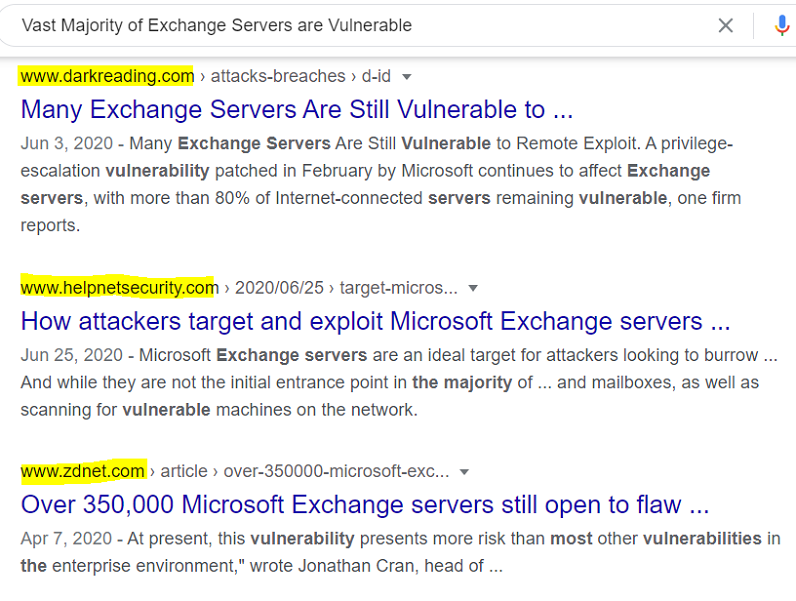
\includegraphics[width=0.45\textwidth]{cyber-feed-info.PNG}\label{fig:cyber-feed-info}}}\hspace{1em}
  \subfloat["Actionable" Cyber Intelligence for CISO ]{\fbox{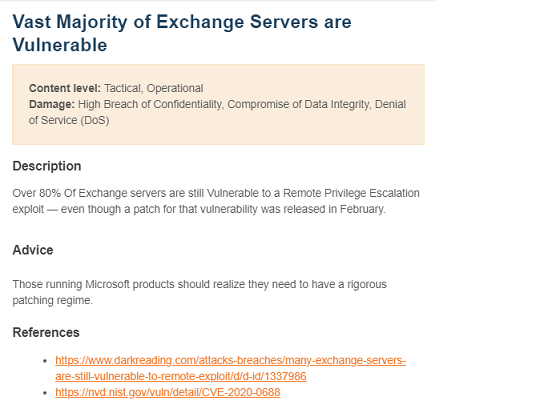
\includegraphics[width=0.45\textwidth]{cyber-feed-intel.PNG}\label{fig:cyber-feed-intel}}}
  \caption{"Scattered \& Raw" vs "Actionable" cyber newsfeed}
\end{figure}


The current status quo is that cyber news or cyber information are being pushed via multiple media \enquote{RSS, mail, WWW, news feeds etc} to multiple organisational stakeholders in a scattered way \citep{schales2011stream}
and are manually interpreted, 
this causes a dilute and incomplete picture 
\citep{liao2016acing}. 
Especially in a world where threats emerge in numbers and sophistication. In 2018 there were one billion unique malware samples counted \citep{kucuk2020deceiving}.
 
 
%\begin{figure}[ht]
%    \centering
%    \fbox{
\includegraphics[width=0.4\linewidth]{Figures/problem2.png}}
%    \caption{Problem with information from multiple feeds. }
%    \label{fig:problem2}
%\end{figure}



% \bigbreak

%----------------------------------------------------------------------------------------

\section*{The Solution: Cybernewsfeed Technology }

To deal with the volumetric cyber newsfeed information, the artefact \enquote{Cybernewsfeed Technology: REVEAL} was build. The design of the artefact is based on literature research on existing threat intelligence tools and users requirements from ON2IT.

The artefact is a software prototype and is created by applying Creative process
\citep{mednick1962associative}.
This artefact collects, processes and transforms cyber newsfeeds into actionable and organisation-specific valuable data. The data aids security professionals in making better decisions.

The artefact helps  organizations getting organisation-specific  actionable  cyber newsfeeds. 
%--------------------------------------

%We build an artefact to see, if we could overcome the volumetric problem. To design the artefact, a literature research was done on existing capability of the threat intelligence platforms and then, the requirements of an ideal system were explored with the cyber security experts. The gaps found between the existing threat intelligence system and the required system was addressed. A new artefact prototype \enquote{Cybernewsfeed Technology: REVEAL} was build and validated. 

\subsection*{Prototype requirement, design and validation}

The first iteration of the requirements for the artefact prototype was collected with the help of ON2IT team. If the reader wants to see the list of requirements, these requirements are are mentioned in TABLE  \ref{tab:requirement-appendix} of Appendix \ref{AppendixA}.

Based on the feedback of the Focus group, I concluded that It is very important to add context and meaning to the cyber information so that it transforms to a cyber intelligence (See FIGURE  \ref{fig:problem-context}).
 

%\subsubsection*{Requirement}\label{Requirement_ES}

%The artefact required some extra code and business logic to filter the relevant cyber newsfeed, some Graphical User Interface (GUI) to interact with cyber newsfeed data and some mechanism to adjust the configurable parameters. In addition to these requirements, the cyber newsfeed data sources needs to kept regularly sanitized.
%Some requiremens needed involvements of human intervention, for example, to perform detail analyis, to add advisory information, and to able to perform editorial checks before shipping to stakeholders. The above requirements would make the cyber newsfeed information not only intelligent but also actionable.

%\subsubsection*{Solution design}

%Based on the requirement mentioned in above section 
%(\nameref{Requirement_ES}), 
%I started exploring existing open source tools to find the capabilities mentioned in section 
%(\nameref{Requirement_ES}). 
%After assessment of 23 different open source tools based on the assessment parameters in mentioned table \ref{table:assessment}, 
%I selected one tool for further customisation and development. 
%The solution artefact is build on top of this open source tool\footnote{Tool used in this thesis for cyber newsfeed collection \url{https://freshrss.org/}} and is made of three modules. 
%These modules comprise of processes, 
%activities and tools at implementation level. 
%The demo of these modules have shown the capability to transform a scattered cyber raw information into an actionable cyber intelligence.

%
\begin{table}
    \caption{Assessment Parameters for tool selection}
    \label{table:assessment}
    \centering{}
   \resizebox{0.75\textwidth}{!}{
    \begin{tabular}{|>{\columncolor[HTML]{ECB4E8}}l|l|}
    \toprule
      \rowcolor[HTML]{BFCEED} 
    
    \textbf{Assessment Parameters} & \textbf{Focus}\\
    \midrule
    Distribution & Open Source\\
    Application Support Forum  Available? & Ease of trouble shoot\\
    Application Active Since years & Old and stable\\
    Application's Last Issue resolved date & Most recent is better\\
    Functional Features &	More is better\\
    Database and GUI & User Friendly\\
   \bottomrule
 
    \end{tabular}
}
\end{table}



%\begin{figure}[ht]
%    \centering
%    \fbox{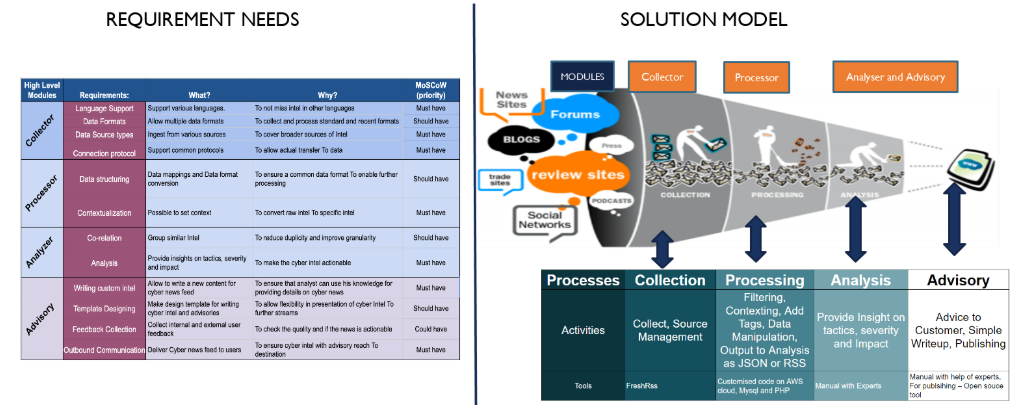
\includegraphics[width=1\linewidth]{Figures/requirement-solution.PNG}}
%    \caption{Requirement versus Solution design}
%    \label{fig:requirement-solution}
%\end{figure}

%\subsection*{Prototype Validation}

The created artefact was validated by the six members of the Focus Group and a CEO of a Cyber security company.

%\section*{Conclusion }



As confirmed by the Focus group participants, 
an  organization-specific cyber newsfeeds can be delivered to an organisation, by configuring the artefact. 
The output newsfeed from this artefact is complemented with the advisory of actionable steps based on the cyber newsfeed content
(see FIGURE \ref{fig:problem-context}).

\begin{figure}[ht]
    \centering
   \fbox{ 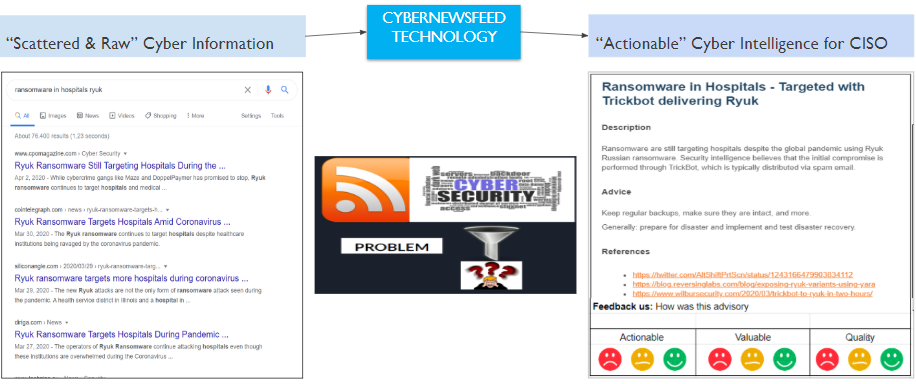
\includegraphics[width=1\linewidth]{Figures/problem-context.PNG}}
    \caption{Cybernewsfeed Technology attempt to address the issue}
    \label{fig:problem-context}
\end{figure}

The results of thesis has been rated useful both in term of its academic purpose and practical use by the stakeholders. The main highlight of this thesis is a demo video, depicting  the academic and rigor concepts being implemented.







